\documentclass[10pt,aspectratio=169]{beamer}

\usetheme{Warsaw}
\usepackage{lmodern}
\usepackage[sfdefault,light,lining]{FiraSans}
\usepackage{xcolor}
\usepackage{booktabs}
\usepackage{tikz}
\usetikzlibrary{positioning,arrows.meta}
\usepackage[utf8]{inputenc}
\usepackage{tabularx} % For wrapping long text columns
\usepackage{caption}


% --- Style Guide Colors [cite: 1] ---
\definecolor{LogicBlue}{RGB}{204,0,0}
\definecolor{InferenceRed}{RGB}{212,55,59}
\definecolor{linkblue}{HTML}{0066FF}
\definecolor{LiteRed}{RGB}{248,232,232}

\setbeamercolor{structure}{fg=InferenceRed}
\setbeamercolor{frametitle}{bg=LogicBlue,fg=white}
\setbeamercolor{palette primary}{bg=LogicBlue,fg=white}
\setbeamercolor{palette secondary}{bg=InferenceRed,fg=white}
\setbeamercolor{block title}{bg=LogicBlue,fg=white}
\setbeamercolor{block body}{bg=LiteRed,fg=black}

\setbeamerfont{page number in head/foot}{size=\large}
\setbeamertemplate{footline}{
  \hfill
  \usebeamercolor[fg]{page number in head/foot}
  \usebeamerfont{page number in head/foot}
  \insertframenumber\,/\,\inserttotalframenumber\kern1em
  \vbox{\vskip6pt}
}


\title{Shaky structures: The wobbly world of causal graphs in software analytics}
\subtitle{Hallunications?  Worse than you think}
\author{Jeremy Hulse (NCSU)\\Nasir U. Eisty (U.Tennesse) \\Tim Menzies (NCSU) }
\institute{prof, cs, \textbf{ncstate}, usa \\ \url{http://timm.fyi} \\~\\\large 
{\bf EMSE}, 30(142), 2025, https://doi.org/10.1007/s10664-025-10690-6  \\
{\bf SLIDES}:
http://timm.fyi/26cause.pdf}
\date{Apr 2025}

% --- Force QR Code to Top Layer ---
\addtobeamertemplate{frametitle}{}{
  \begin{tikzpicture}[remember picture,overlay]
    \ifnum\insertframenumber>1
      \node[anchor=north east, xshift=0mm, yshift=2mm] 
        at (current page.north east) 
        {
\includegraphics[width=20mm]{qrcode_timm.fyi.png}};
    \fi
  \end{tikzpicture}
}

\begin{document}

% 1. TITLE SLIDE
\begin{frame}
\titlepage
\end{frame}

% 2. MOTIVATION (The Hype)
\begin{frame}{Claim: Causal graph generations not a source of "truth"}

\begin{itemize}
    \item \textbf{We don't want} to know that "Size correlates with Defects."
    \item We want to know: "If I change this module, will I stop the bugs?"
    \item Causal Discovery Algorithms (CDAs) promise to find these hidden structures automatically.
    \item But... suffer from \textbf{mass hallunication.}
\end{itemize}

\vspace{3mm}
\end{frame}

\begin{frame}[plain]
    \begin{tikzpicture}[remember picture,overlay]
        \node[at=(current page.center)] {
            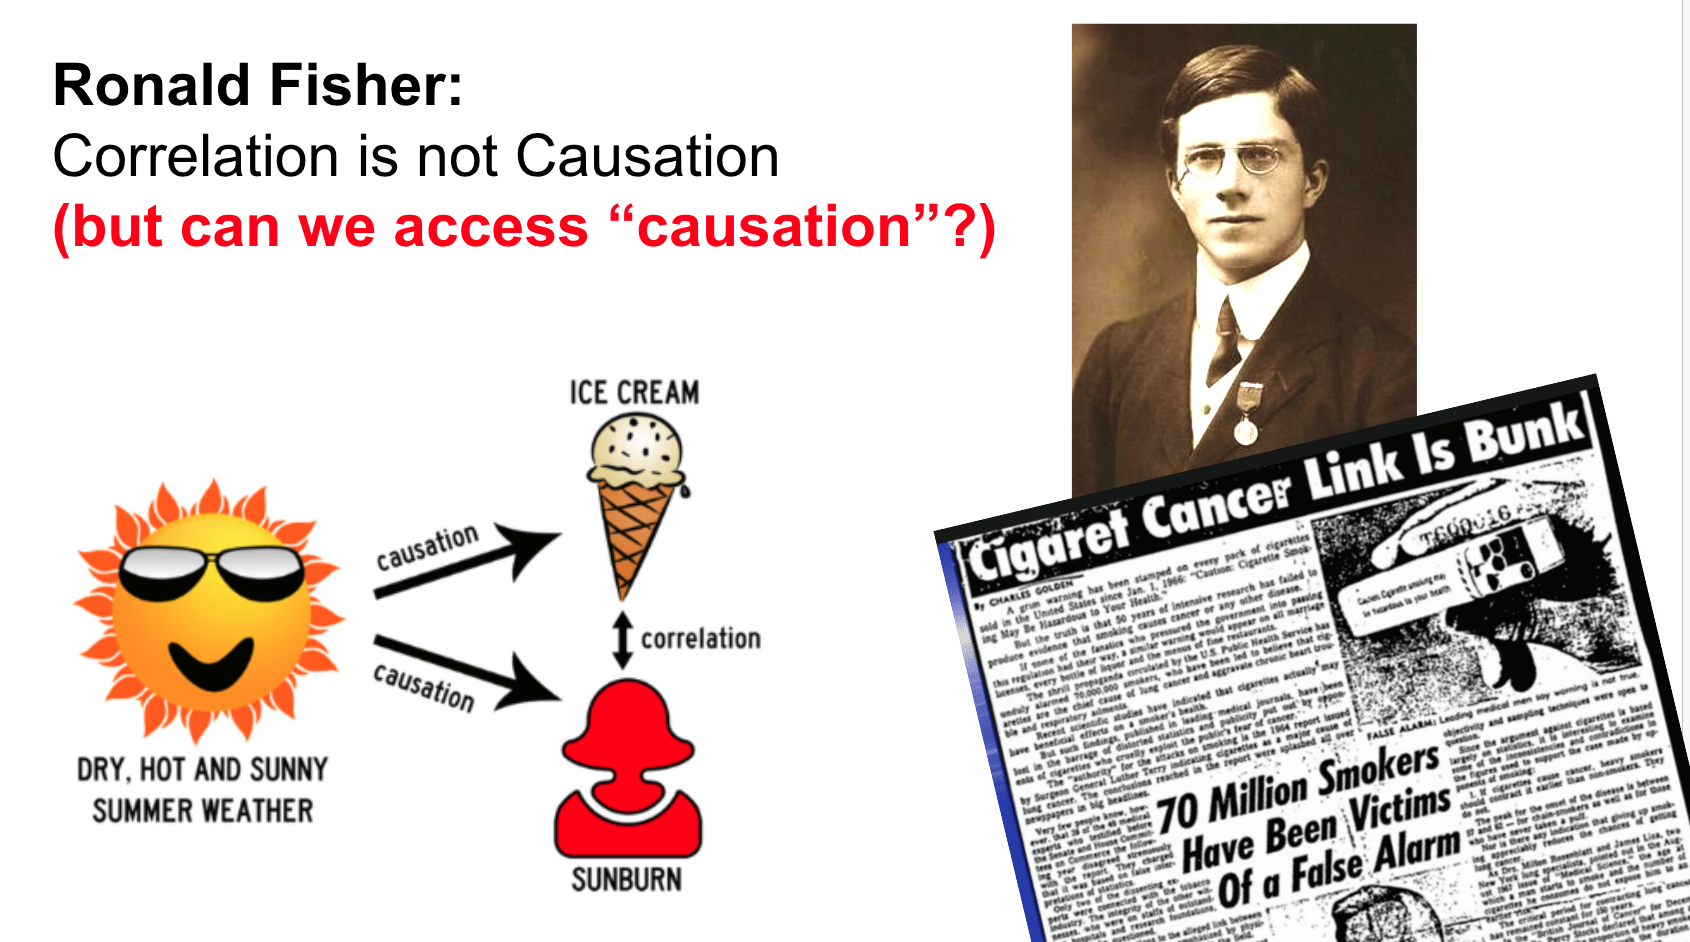
\includegraphics[height=\paperheight]{correlation.png}
        };
    \end{tikzpicture}
\end{frame}

\begin{frame}[plain]
    \begin{tikzpicture}[remember picture,overlay]
        \node[at=(current page.center)] {
            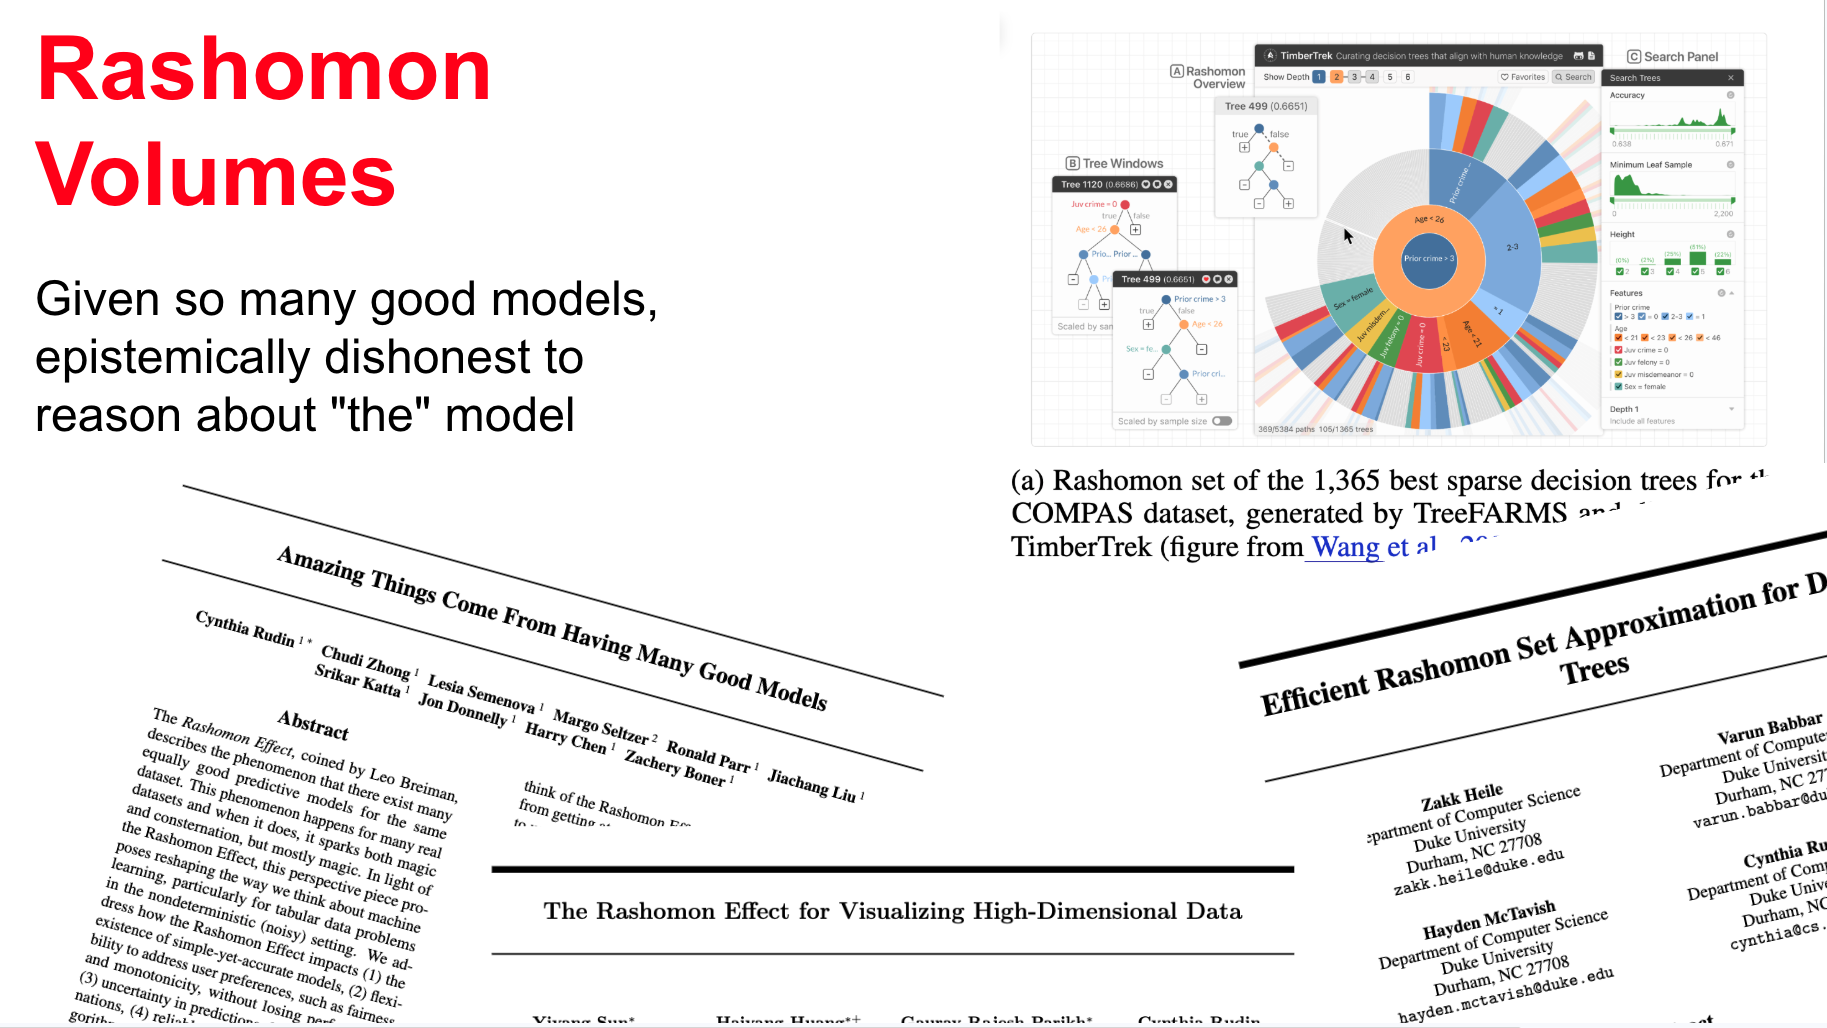
\includegraphics[height=\paperheight]{rash.png}
        };
    \end{tikzpicture}
\end{frame}


% 3. THE CORE PROBLEM (The Reality)
\begin{frame}{The Reality: The Instability Problem}
  \textbf{Claim:} Causal graphs generators:  \textbf{too unstable }to trust.

\vspace{3mm}
\begin{block}{The Definition of Instability}
Small changes to the data result in \textbf{large, unpredictable changes} in the resulting graphs.
\end{block}

\vspace{3mm}
\begin{itemize}
    \item If the graph changes every time you re-run it, it isn't an "explanation."
    \item It is just\textbf{ noise masquerading }as a diagram.
\end{itemize}

Four most prominent paradigms in causal discovery: all hallunicate

~\\

\centering
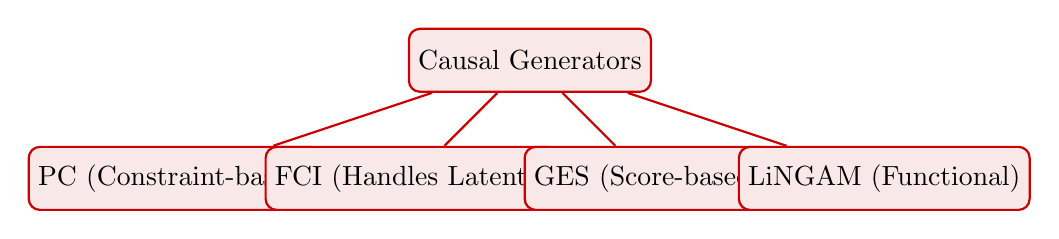
\begin{tikzpicture}[
  box/.style={draw=LogicBlue, rounded corners, thick, fill=LiteRed, minimum width=2.2cm, minimum height=0.8cm},
  line/.style={draw=LogicBlue, thick}
]
\node[box] (cda) at (0,1.5) {Causal Generators};
\node[box] (pc) at (-4.5,0) {PC (Constraint-based)};
\node[box] (fci) at (-1.5,0) {FCI (Handles Latents)};
\node[box] (ges) at (1.5,0) {GES (Score-based)};
\node[box] (lin) at (4.5,0) {LiNGAM (Functional)};

\draw[line] (cda) -- (pc);
\draw[line] (cda) -- (fci);
\draw[line] (cda) -- (ges);
\draw[line] (cda) -- (lin);
\end{tikzpicture}

\end{frame}

% % 5. EXPERIMENTAL DESIGN: THE CORPUS
% \begin{frame}{The Archive: 23 Datasets across 30 Years}
% \begin{itemize}
%     \item We didn't test on toy data. We used the \textbf{PROMISE} and \textbf{JURECZKO} repositories.
%     \item \textbf{Breadth:} Ant, Camel, JEdit, Lucene, POI, Tomcat, Velocity, and more.
%     \item \textbf{Depth:} Multiple releases per project (e.g., Ant 1.3, 1.4, 1.5, 1.6, 1.7).
% \end{itemize}
%
% \vspace{3mm}
% \begin{block}{Not a green-field project}
% This is a audit of how these tools behave on real-world SE evolution. [cite: 11]
% \end{block}
% \end{frame}
%
% 6. METRIC: HOW WE MEASURE INSTABILITY
\begin{frame}{Hallunications in SE (Causal graphs)}

  \vspace{3mm}
\begin{itemize}
  \item $J(A,B) = \frac{|E_A \cap E_B|}{|E_A \cup E_B|}$
  \item $J=1.0$: The graphs are \textbf{identical}.
    \item $J=0.0$: The graphs have zero edges in common.
    \item \textbf{Rule:} If $J$ is low, your "Why Engine" is broken. [cite: 25]
\end{itemize}

\small
We measured Jaccard across versions, across tools, and across data subsets. e.g. v5,v7:

      \begin{minipage}{2.1in}
  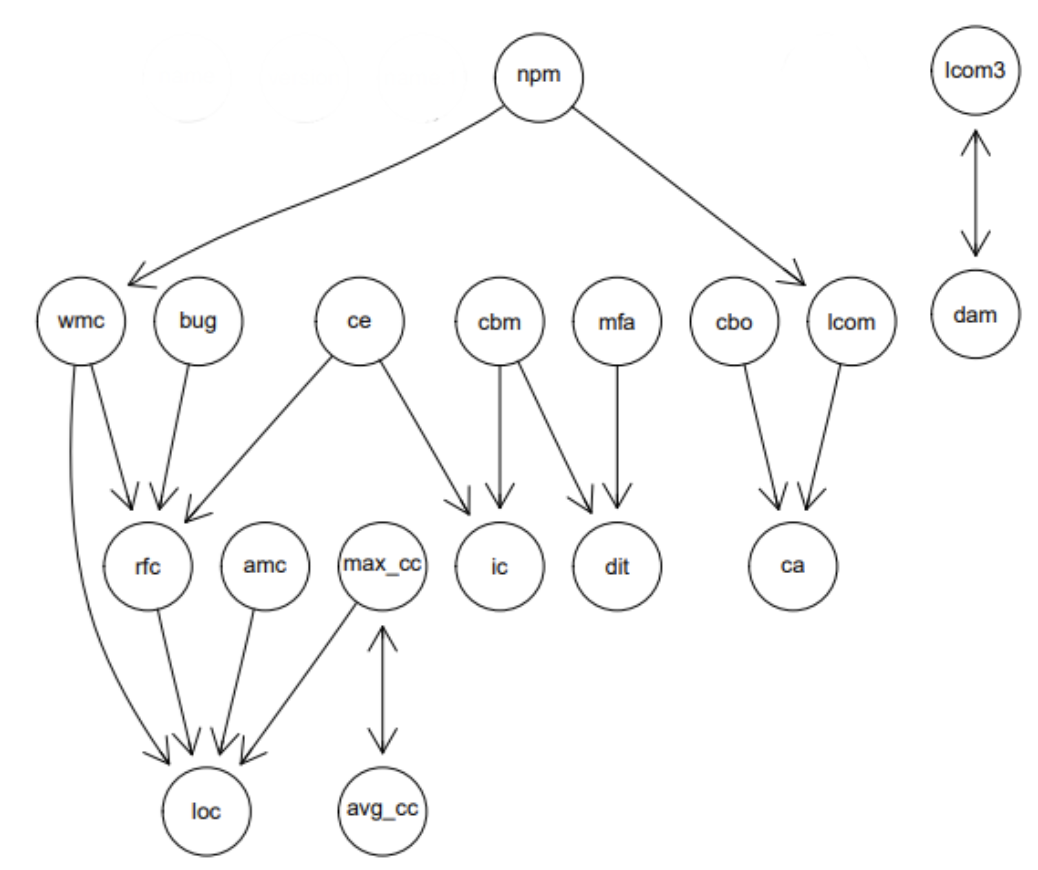
\includegraphics[height=4.5cm]{one.png}
\end{minipage}\begin{minipage}{2.2in}
  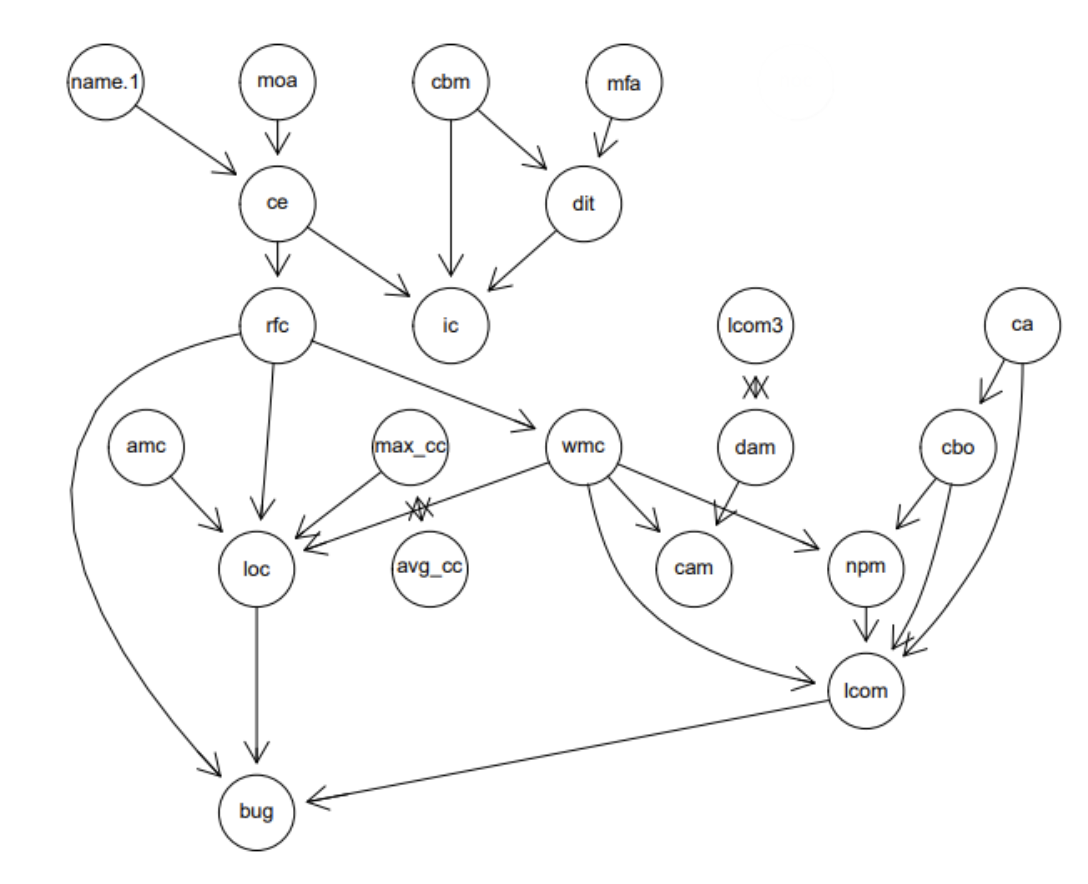
\includegraphics[height=4.5cm]{two.png}
\end{minipage}\begin{minipage}{2.2in}
  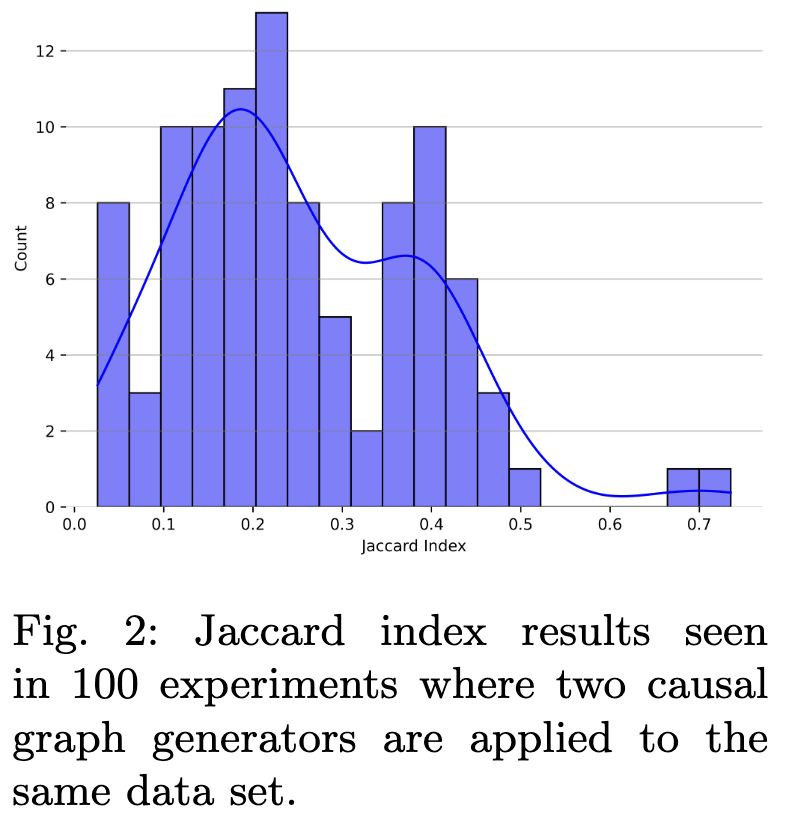
\includegraphics[height=4cm]{three.png}
\end{minipage}

\end{frame}

\begin{frame}{Hallunications in SE (regression, effort estimation)}
20 times,
\begin{itemize}
  \item \textbf{Select} 66\% of the data;
\item Learn model {\em effort} $= \beta_0 + \beta_1x_1 + \beta_2x_2 +...$
\item Show the \textbf{sorted} $\beta_i$ values.
\end{itemize}

\begin{center}
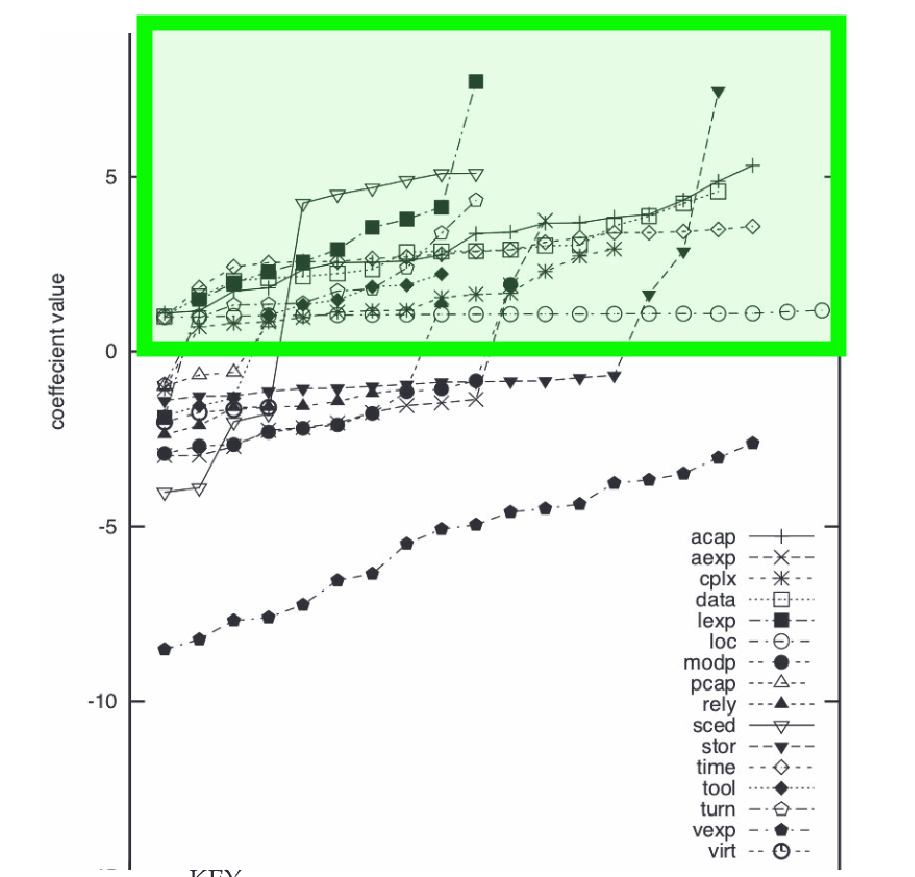
\includegraphics[height=2.25in]{corr.pdf}
\end{center}
\end{frame}

\begin{frame}{Hallunications in SE (defect prediction)}

In 28 publications:
\begin{itemize}
\item 
  Is feature X postively or negatively \textbf{correalted} to defects?
\end{itemize}

\begin{center}
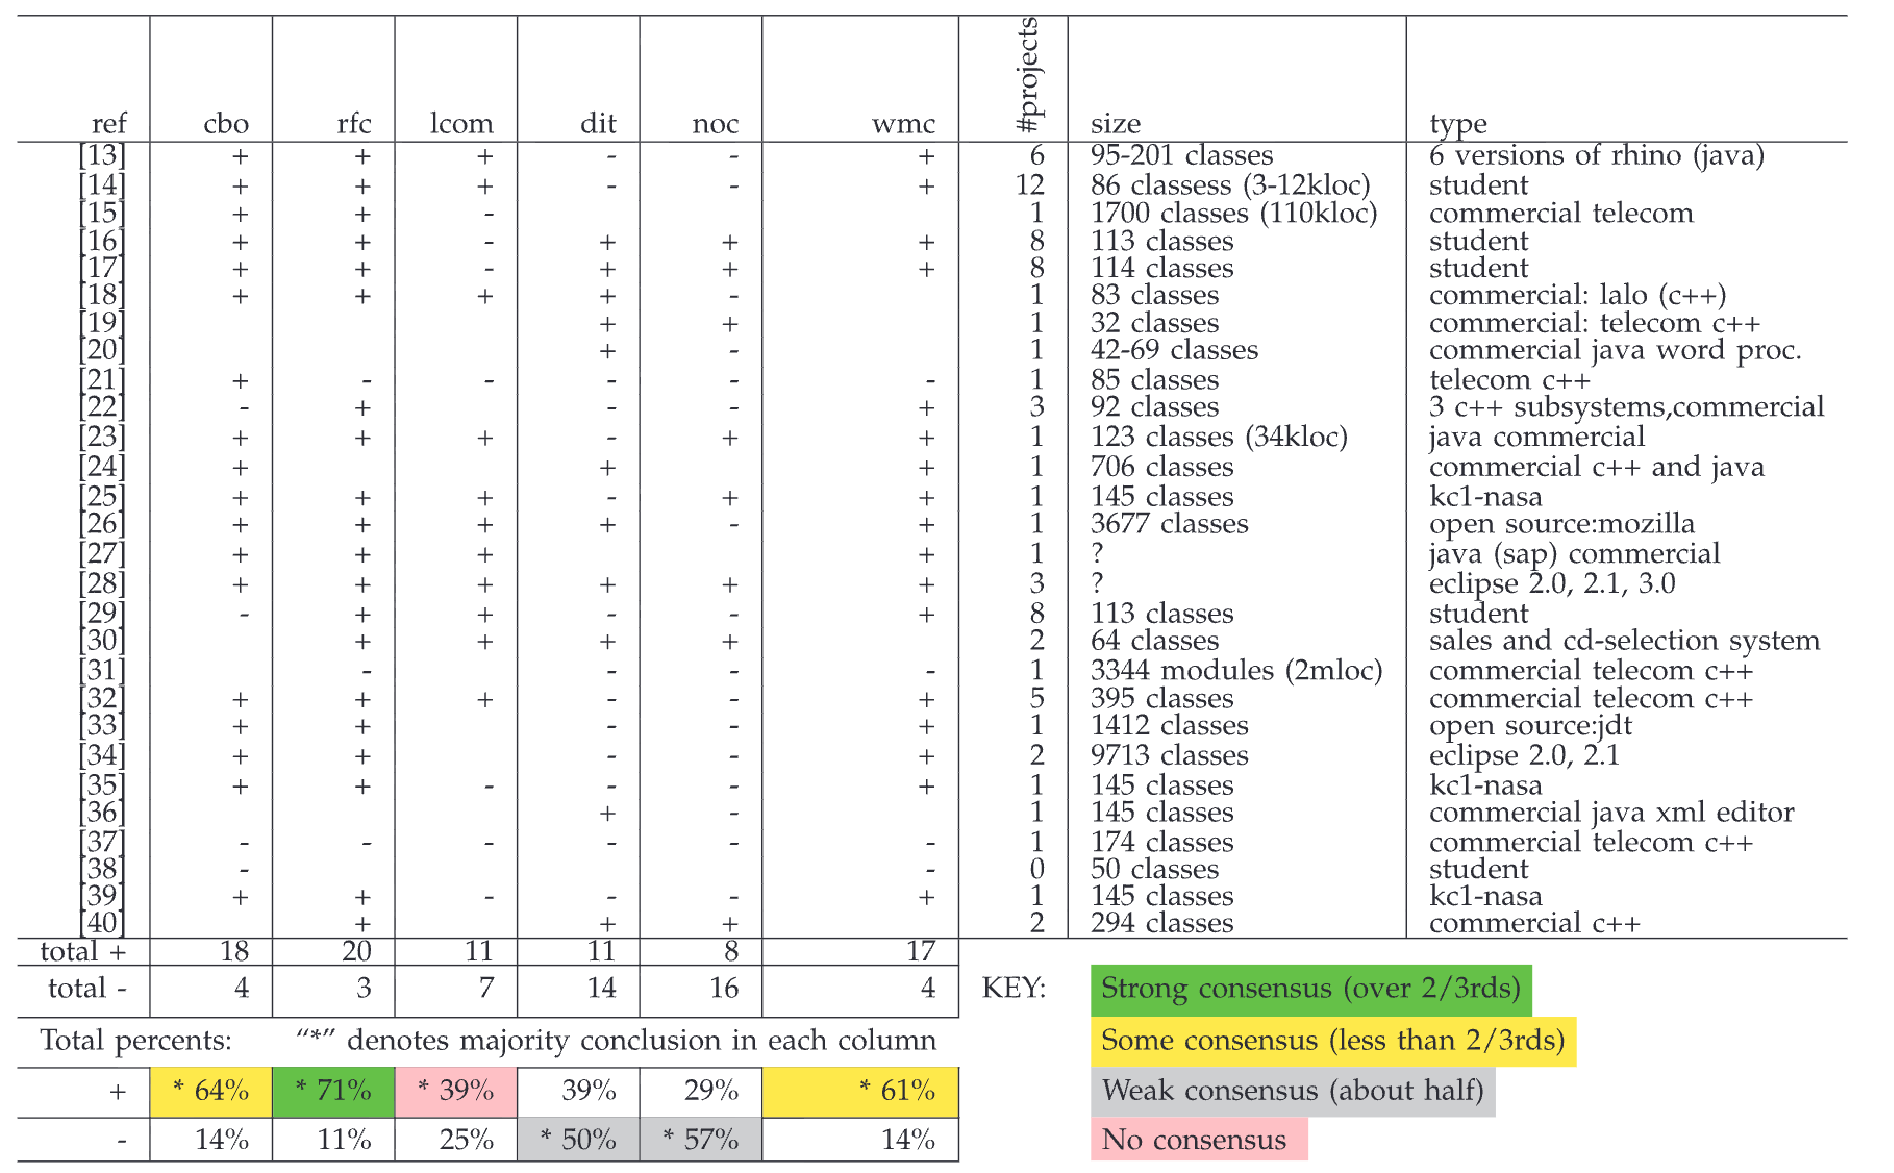
\includegraphics[height=2.5in]{defect.pdf}
\end{center}
\end{frame}



\begin{frame}{Hallunications in SE (topic modeling)}
Groups of words (topics) seen in Stackoverflow:
\begin{itemize}
  \item Two runs, \textbf{shuffle} row order in-between;
\item Column1 = percent of words in run1's topics appearing in\textbf{ run2's topics
}\end{itemize}



    {\footnotesize % Reduces font size to fit more data
    \renewcommand{\arraystretch}{1.1} % Slightly tighter row spacing
    
    \begin{columns}[T]
        % Left Column
        \begin{column}{0.48\textwidth}
            \begin{tabularx}{\textwidth}{l p{2.5cm} X}
                \toprule
                \textbf{\%} & \textbf{Topic} & \textbf{Top Words} \\
                \midrule
                100 & Xaml Binding & grid window bind... \\
                100 & Ruby on Rails & rubi rail gem lib... \\
                100 & MVC & http com java... \\
                88  & Objective C & self cell nsstring... \\
                88  & Func. Returns & function const char... \\
                77  & Testing & chang tri work use... \\
                77  & Socket Comm. & Main send socket... \\
                77  & Q and A & know need want... \\
                77  & OO Prog. & instanc void type... \\
                77  & HTML Links & com http www url... \\
                \bottomrule
            \end{tabularx}
        \end{column}

        % Right Column
        \begin{column}{0.48\textwidth}
            \begin{tabularx}{\textwidth}{l p{2.5cm} X}
                \toprule
                \textbf{\%} & \textbf{Topic} & \textbf{Top Words} \\
                \midrule
                77  & Display & height jpg imag... \\
                66  & Windows Tips & studio net dll web... \\
                66  & Website Des. & left span style text... \\
                66  & Web Dev. & script jqueri func... \\
                66  & Java Prog. & java void new... \\
                66  & Date/Time & select day valu... \\
                66  & Database & column order group... \\
                66  & Android View & height content text... \\
                66  & .NET Frame. & net form text check... \\
                55  & iOS App Dev. & applic user need... \\
                \bottomrule
            \end{tabularx}
        \end{column}
    \end{columns}}
    

\end{frame}


% 7. FINDING 1: INTRA-PROJECT (TIME)
\begin{frame}{Finding 1: The Time Flip in defect prediction data}
\textbf{Question:} Does the "cause" of defects stay the same from Version 1 to Version 2?

\vspace{3mm}
\begin{itemize}
    \item \textbf{The Result:} In nearly all cases, over half the edges vanish between releases.
    \item Median stability across versions: \textbf{Extremely Low}.
    \item \textbf{The Risk:} A manager fixes a "cause" in Version 1.5 that no longer exists in Version 1.7.
\end{itemize}

\begin{center}
  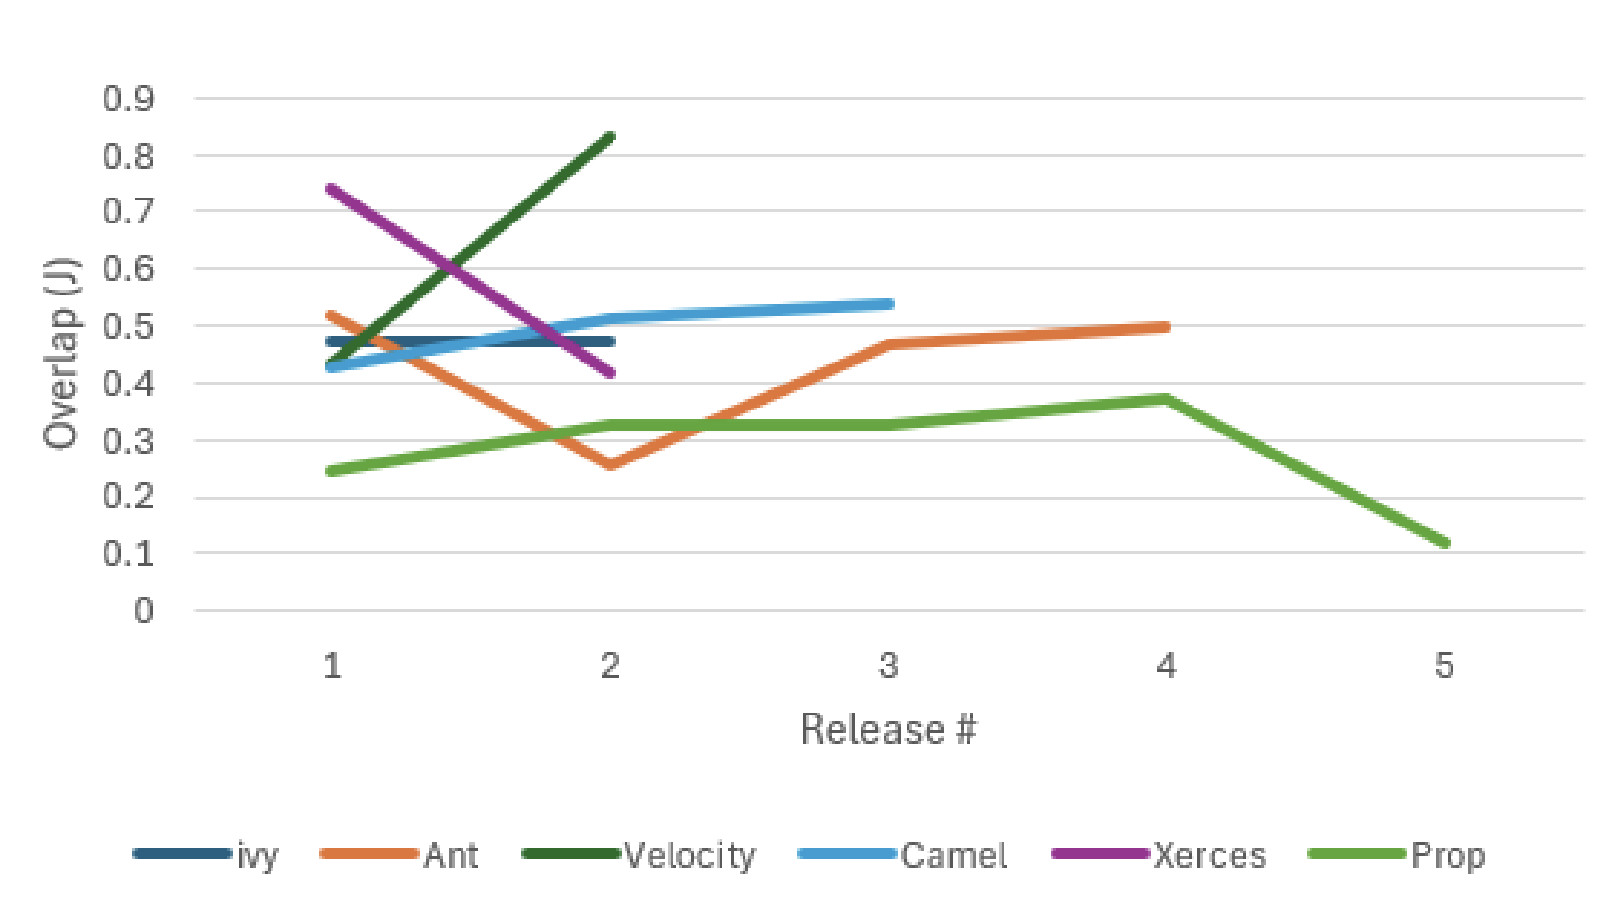
\includegraphics[height=4cm]{rq1.png}
\end{center}

\end{frame}

% 8. FINDING 2: INTER-PROJECT (DOMAIN)
\begin{frame}{Finding 2: The Domain Gap}
\textbf{Question:} If I learn the causal graph for Camel, can I use it for Tomcat?

\vspace{3mm}
\begin{itemize}
    \item \textbf{The Result:} Over two-thirds of causal connections differ between projects.
    \item This suggests causal discovery in SE is \textbf{highly idiosyncratic}.
    \item Generalization is a dangerous assumption in this landscape.
\end{itemize}

~\\

\begin{center}
  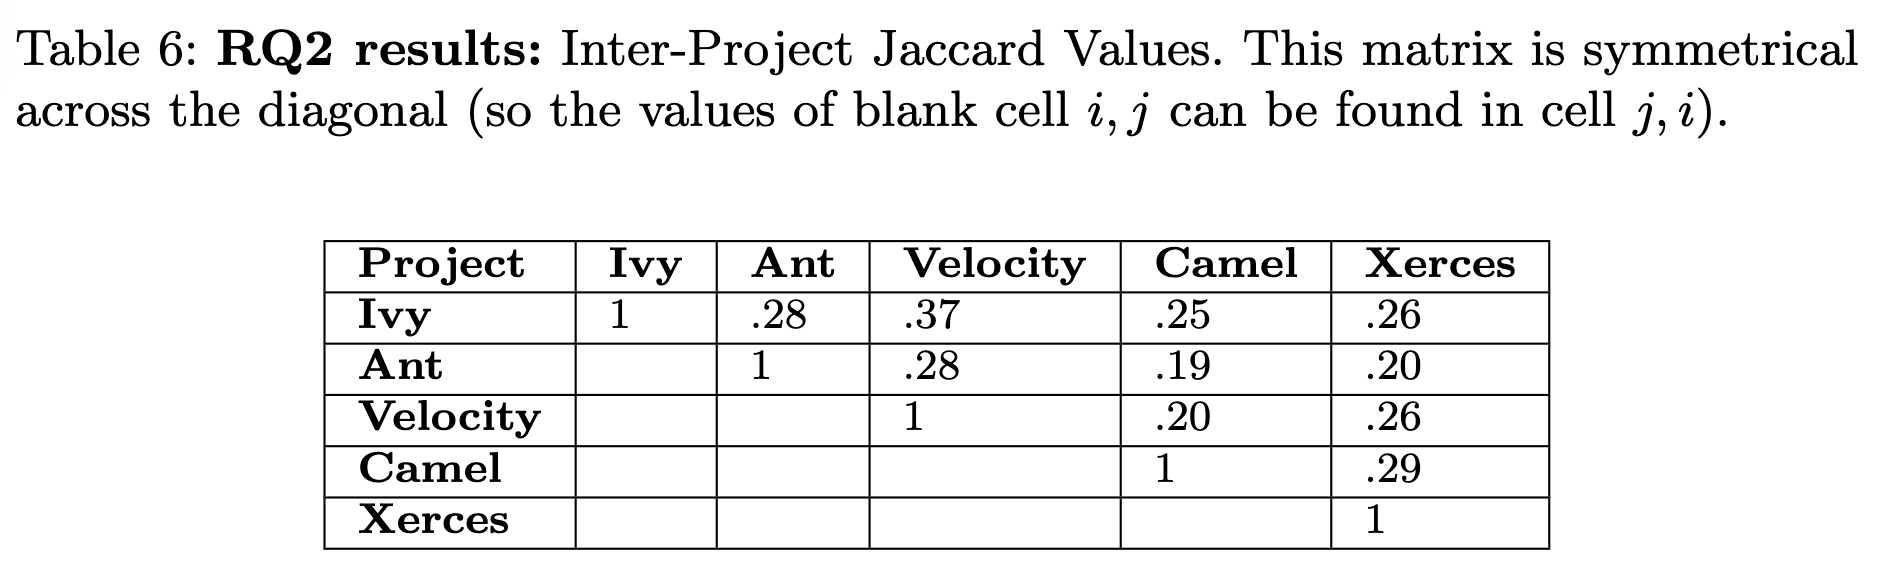
\includegraphics[height=3cm]{cross1.png}
\end{center}

\end{frame}
% 10. FINDING 4: PARAMETER SENSITIVITY
\begin{frame}{Finding 3: The Fragility of Alpha}
\textbf{Question:} Does graph change with changing significance level $\alpha$ (e.g., 0.01 to 0.05)?

\vspace{3mm}
\begin{itemize}
    \item \textbf{The Result:} Minor tuning adjustments generate radically different causal structures.
    \item These tools are \textbf{not robust} to standard hyperparameter variations.
\end{itemize}


 \begin{minipage}{2in}
  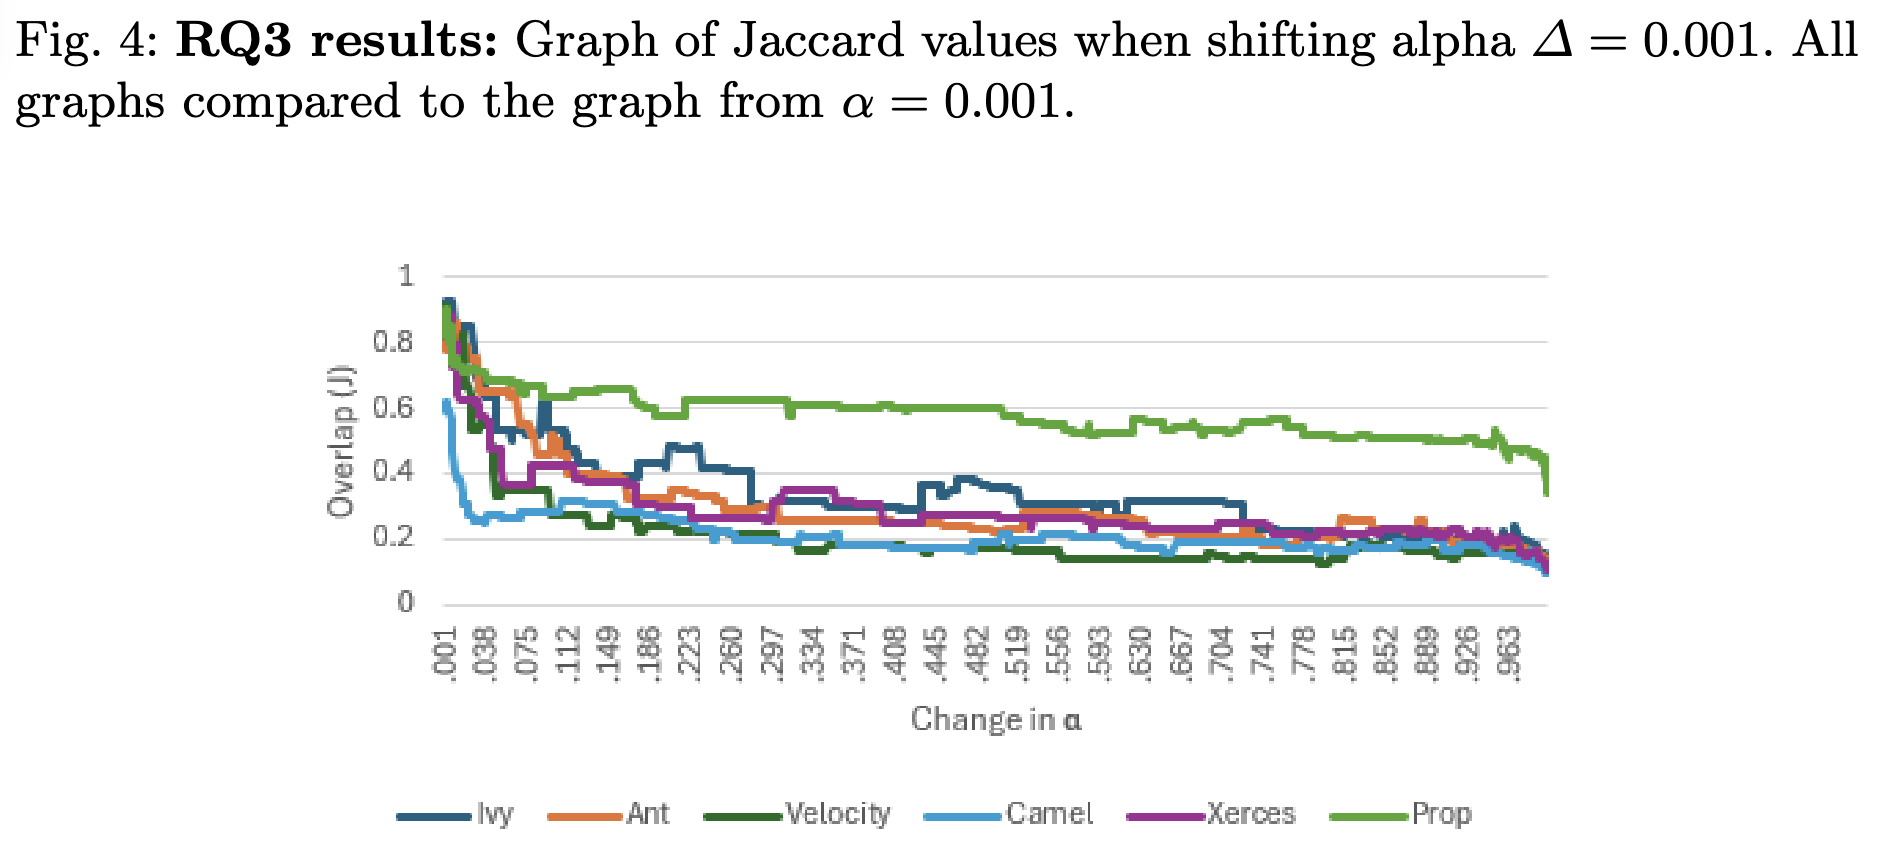
\includegraphics[height=6cm]{alpha.png}
  \end{minipage}


\vspace{3mm}
\begin{block}{Key Design Warning}
If your "Why" depends on whether $\alpha=0.01$ or $0.05$, you don't have a "Why." [cite: 25]
\end{block}
\end{frame}

% 11. FINDING 5: DATA SENSITIVITY (THE 10% TEST)
\begin{frame}{Finding 5: Other Data? Other Causal Generators?}
\begin{center}
  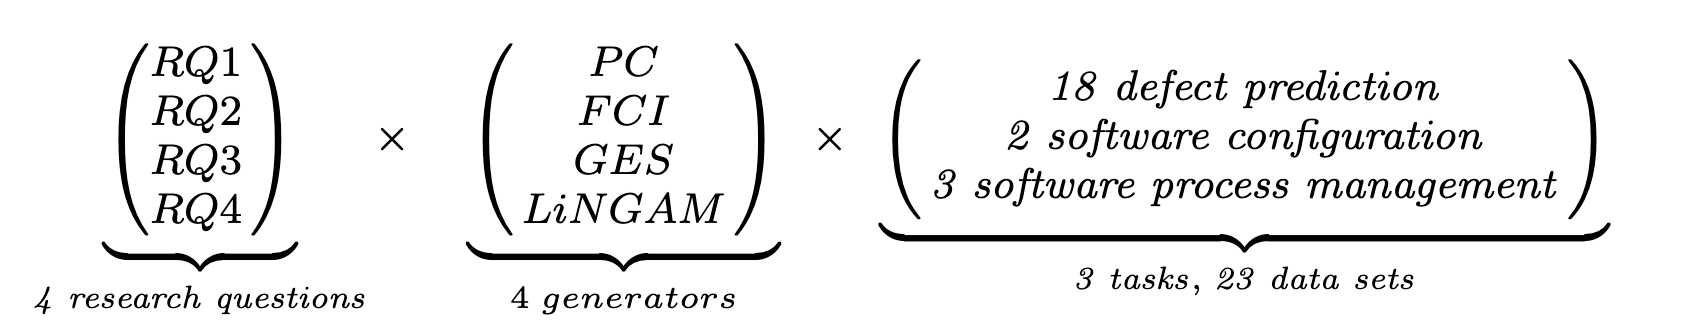
\includegraphics[height=2cm]{rqs.png}


  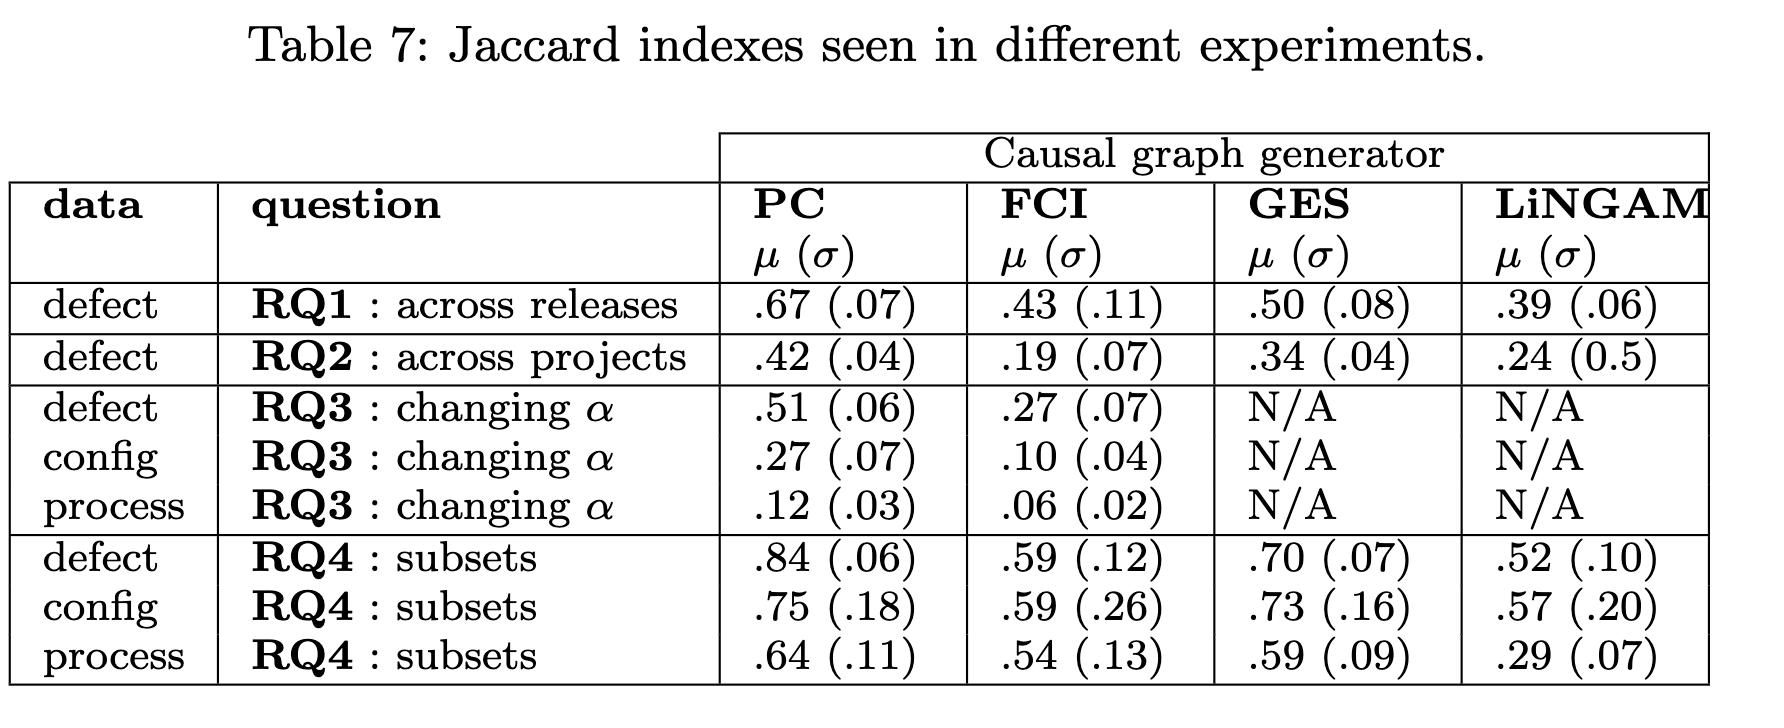
\includegraphics[height=4.5cm]{rqs1.png}
\end{center}

\end{frame}

% 12. DISCUSSION: WHY IS SE SO HARD?
\begin{frame}{The Why: Why Do Graphs Fail in SE?}
\begin{itemize}
    \item \textbf{Data Sparsity:} SE data is often "fat and short" (many features, few rows). [cite: 9]
    \item \textbf{Noisy Metrics:} Static code features are proxies, not direct physical laws.
    \item \textbf{Stochastic Nature:} Software evolution is driven by human choice, not just mathematical necessity. [cite: 37]
\end{itemize}

\vspace{3mm}
\small
We need \textbf{hybrid workflows} that combine these graphs with symbolic checks. [cite: 5, 25]
\end{frame}

% 13. ROADMAP TO STABILITY
\begin{frame}{Roadmap: Moving Beyond the "Hype"}
\begin{enumerate}
    \item \textbf{Intersection Filters:} Only report edges found by \textit{at least two} different generators.
    \item \textbf{Stability Audits:} Always run a "10\% drop test" before publishing a graph.
    \item \textbf{Type-Safe Checks:} Use Z3 to reject causal links that violate known SE constraints. [cite: 14, 25]
    \item \textbf{Ensemble Causality:} Treat causal discovery as an optimization problem over an ensemble of graphs. [cite: 33]
\end{enumerate}
\end{frame}

% 14. CLOSING PITCH
\begin{frame}{Conclusion}
\begin{itemize}
    \item  Causal graphs are a powerful \textbf{hypothesis generator}, but a dangerous \textbf{decision maker}—until we solve the instability problem.
\end{itemize}

\vspace{4mm}
\begin{block}{Closing pitch}
  The hallunication problem is much \textbf{worse} than you think.
\end{block}

\end{frame}

\begin{frame}[plain]
    \begin{tikzpicture}[remember picture,overlay]
        \node[at=(current page.center)] {
            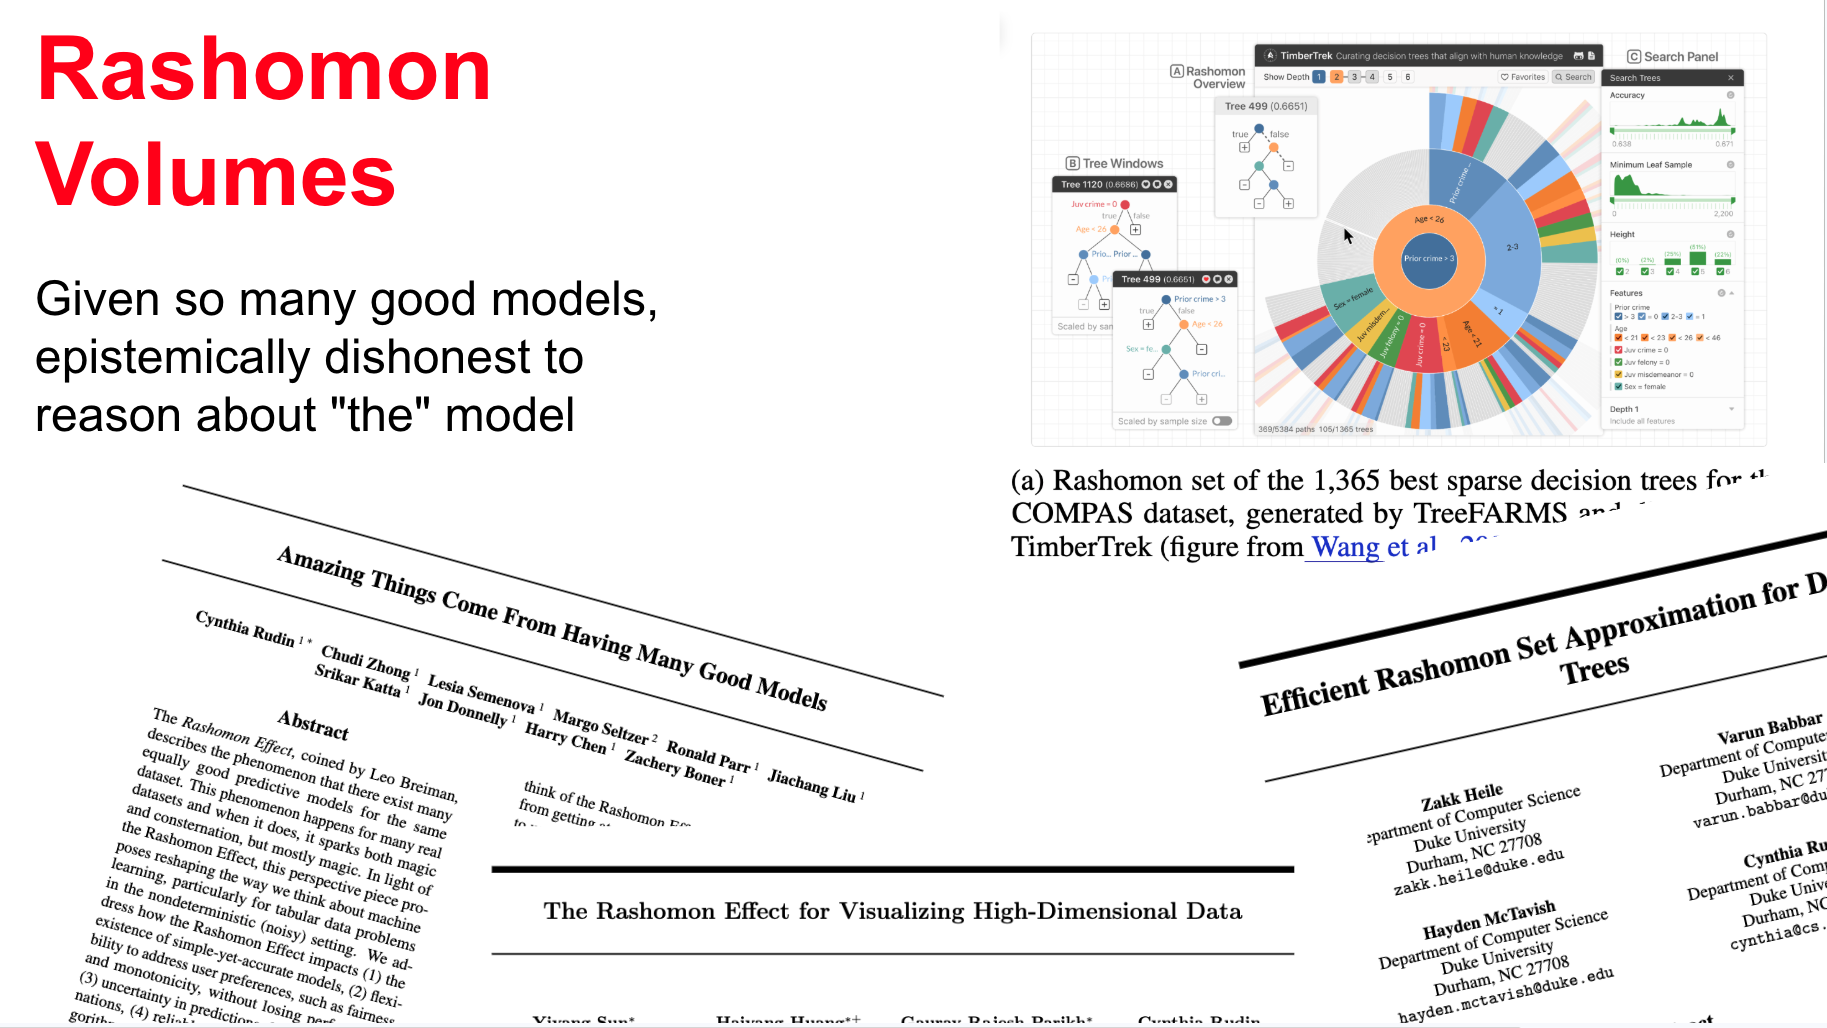
\includegraphics[height=\paperheight]{rash.png}
        };
    \end{tikzpicture}
\end{frame}


\end{document}
